%%% PRACE GENERIC LAYOUT; DO NOT CHANGE %%%
\documentclass{prace}
%%% END OF PRACE GENERIC LAYOUT %%%

% TITLE
%   - use the name of your project
%   - capitalise the first letter
\title{Initial Design Document}
\date{31.01.2024}

% Instead of a DOI, we will use the name of the club
\doi{CyberSecurity Club at SFSU}

% AUTHORS
\author[1]{Ethan Hanlon}
\author[1]{Michael Petrossian}

% AFFILIATIONS
\affiliation{San Francisco State University, 1600 Holloway Avenue, San Francisco, CA 94132, USA}

%%% PRACE GENERIC LAYOUT; DO NOT CHANGE %%%
\begin{document}
\maketitle
%%% END OF PRACE GENERIC LAYOUT %%%

% ABSTRACT
%   - write a concise abstract that outlines the approach / methods, main 
%     results, and relevance of your project
\begin{abstract}
This research focuses on designing and implementing a secure MISC device that will be built to adhere to the standards of the functional and security requirements. Our design will 
aim to withstand all attack scenarios presented by the MITRE documentation, as well as provide a new approach to embedded system programming with the popular and recent memory-safe Rust programming language. 
\end{abstract}

\section{Introduction}

The aim for this project is to create a device that can communicate securely and validate components for integrity and authenticity.
In developing and implementing a MISC secure medical device, our team found that cryptography
provided the strongest protection against most attack scenarios and fulfilled much of the requirements
that demanded confidentiality, integrity, and authenticity. Although our design appears bullet-proof, there are still
some fundemental flaws that, as will be discussed later, can only be mitigated rather than completely resolved. Our methods of encryption will comprise of elliptic curve key pairs, 
psuedo-random token seeds, and hash digests - all of which can be generated and derived from the build deployment.

\section{Functional Requirements}

\subsection{Build Environment}

For the purpose of preventing bugs and keeping safe coding standards, the Rust programming language will be used.
This will involve improvising the build environment from the design reference so that we can complement Rust's deployment. 

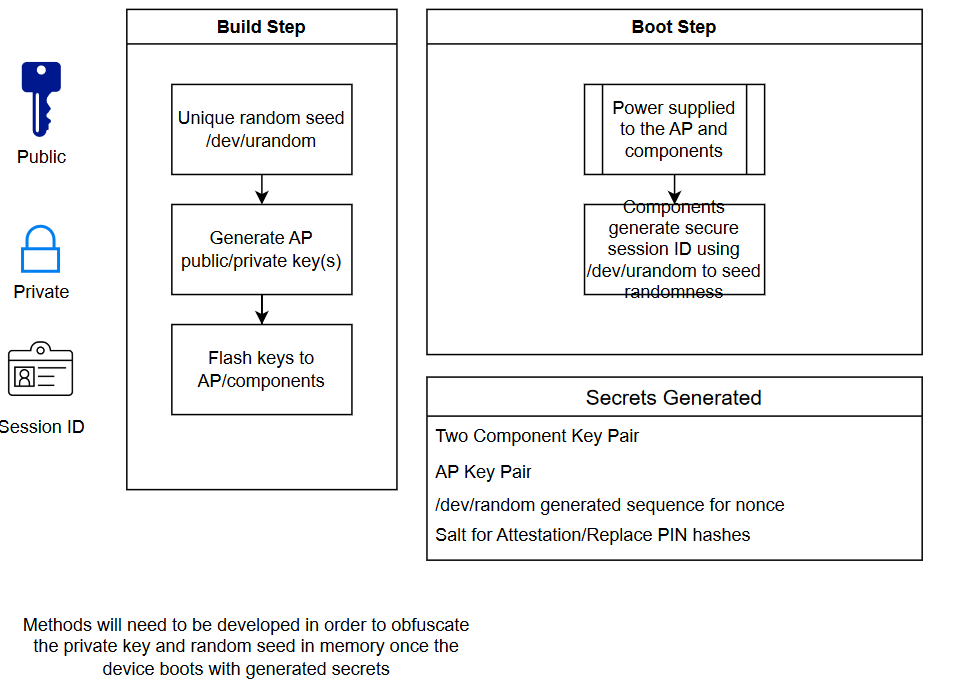
\includegraphics[scale=0.75]{./diagramSR1.png}

\subsection{Attest}

When the authorized user enters the correct PIN, a unique sequence of numbers generated during the build deployment, they will be able to 
retrieve the attestation data through the AP.

\subsection{Replace}

An authorized user with a valid token can change the component ID that the AP is provisioning so long as the device is also provided a new "passcode" that 
will act as the new seed for the device's nonce to sync correctly.

\subsection{Boot}

When the device boots, the AP and Components will verify each other where it will then be ready to communicate between each other for operation

\subsection{Secure Communication}

Same as above. TBD

\section{Security Requirements}

\subsection{Security Requirement 1}
Security Requirement 1 (\textbf{SR1}) requires us to ensure the Application Processor will not boot unless
expected components are present and valid. Our plan for this involves a two-pronged approach
which uses public/private key encryption and a secure cryptographic nonce.

During the build process, we will generate a public/private key pair. The public key will be
flashed onto the components, and the private key will be stored in the application processor.
Additionally, a random seed will be generated using /dev/urandom and will be used to seed the
random generator for both the application processor and component. This seed will be used by the components and the application processor to generate
and validate cryptographic nonces - it will also prevent replay attacks from being performed in case the attacker sets up a MITM and tries to boot the AP using a valid signal but a malicious component.

The components will use the public key to encrypt the nonce along with their own
unique identifier and send it back to the application processor over I2C bus. The application
processor will use the private key to decrypt the nonce and verify that it matches the original
nonce. If the nonces match, a new nonce is generated by the AP and sends out an acknowledgement to the component to continue the boot sequence. If no message is received, or the nonces do not match, the application
processor will not boot.

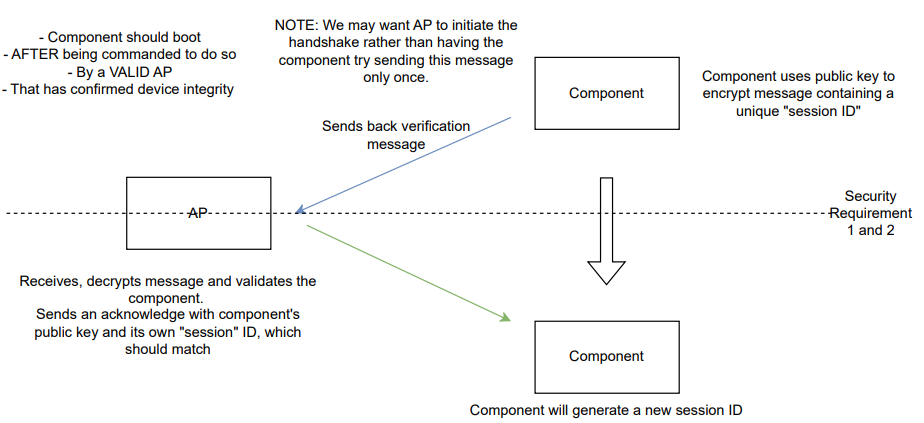
\includegraphics[scale=0.85]{./diagramSR12.png}

\subsection{Security Requirement 2}
Security Requirement 2 (\textbf{SR2}) requires us to ensure that the components will not boot until commanded
to do so by an Application Processor that has validated the integrity of the system. Our plan to
meet this requirement is much the same as the plan for Security Requirement 1, but in reverse.

During the build process, a random number will seed the psuedo-random generator in the firmware as delineated in 
SR1. In addition, each component will receive a public/private key pair similar to the AP's.
This key will be used to encrypt messages before transmitting them over the I2C bus, as well
as to verify digital signatures.

After the application processor verifies the message sent by the components as delineated
in SR1, it will return an acknowledgement, encrypted with the component's public key. Upon
receipt of this acknowledgement, the component will use its private key to decrypt the 
message and validate its digital signature. From there, the nonce will be checked against
the random key generator. If the message is not present, the digital signature is invalid,
or the nonce verification fails, the component will immediately halt the boot process.
Conversely, if all checks pass - suggesting the AP successfully validated the components -
the component will proceed with the boot sequence.

\subsection{Security Requirement 3}

Security Requirement 3 (\textbf{SR3}) Requires that the Attestation PINs and Replacement Tokens are kept confidential.
To accomplish this, we will hash and salt the secrets to prevent the plaintext versions from being exfiltrated.
It's unrealistic, given physical access to the machine, to expect that we can fully prevent the memory holding
the secrets from being extracted from the device. However, by using SHA256, we can make the data useless to the
attacker. By salting the PINs using a special token generated at compile time, we can prevent the use of a rainbow
table to get around the hashing. Only an authorized personal with the secret PIN is able to extract the attestation data.

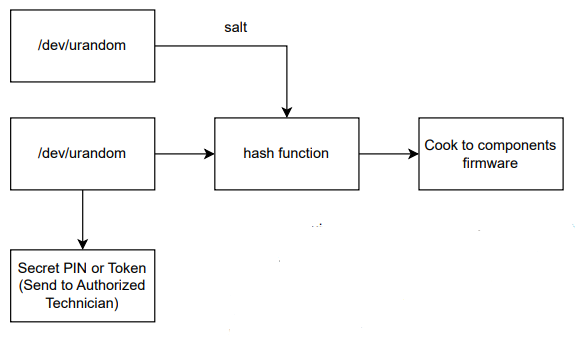
\includegraphics{./diagramSR3.png}

\subsection{Security Requirement 4}

Security requirement 4 (\textbf{SR4}) states that the attestation data is to be kept confidential and secure from unauthorized changes.
 Assuming that an attacker has the ability to modify the data directly, fulfilling this requirement can be done by encrypting 
 the attestation data with the public key of the AP and embedding the data with its hash digest. Whenever an authorized user 
 requests the attestation data, the AP first decrypts the data received by the component and then verifies the integrity by 
 matching the resulting hash of the data with the embedded digest that went along with it. This technique is inspired by modern 
 message authentication with message authentication codes (MAC) ensuring the integrity of data whenever it is in transit.


\subsection{Security Requirement 5}

Security requirement five (SR5) requires us to ensure the integrity and authenticity of all post-boot MISC secure communications. Our 
plan to solve this challenge is to write validation requirements directly into the firmware. All messages bound for the I2C bus will have 
a digest created based on the device's private key, which was generated on the build step for each device for SR1. When a message is received, 
the firmware will first check the message against the digest. If the message fails to validate, we can assume it is either damaged or inauthentic 
and reject it accordingly.

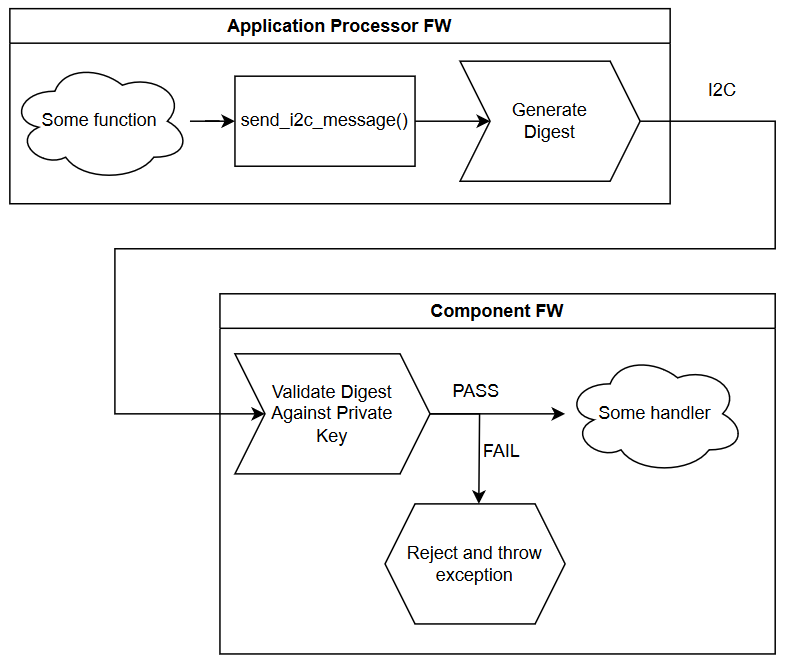
\includegraphics{./diagramSR5.png}

% REFERENCE LIST
%   - use \thebibliography and \bibitems to enter references, no separate .bib
%     files (NOTE FROM MICHAEL : YES WE NEED THIS)
%   - use normal font for *everything* (no bold typefaces etc.)
%   - shorten the last page number, i.e. 51--9 for pages 51--59
%   - for more than 6 authors the first 6 should be listed followed by et al.
%     - use \emph{et al.} for the et al.
%   - end each reference with a period
%
% example:
%   \begin{thebibliography}{99}
%     \bibitem{scholes-DiscussFaradaySoc-70}
%       S. Scholes, Discuss. Faraday Soc. No. 50 (1970) 222.
%     \bibitem{mazurin-Phase-Separation-in-Glass-84}
%       O.V. Mazurin and E.A. Porai-Koshits (eds.), 
%       Phase Separation in Glass, North-Holland, Amsterdam, 1984.
%     \bibitem{dimitriev-JMaterSci-75}
%       Y. Dimitriev and E. Kashchieva, J.Mater. Sci. 10 (1975) 1419.
%     \bibitem{eaton-Porous-Glass-Support-Material-75}
%       D.L. Eaton, Porous Glass Support Material, US Patent No. 3 904 422 
%       (1975).
%   \end{thebibliography}

% \begin{thebibliography}{99}
% 	\bibitem{scholes-DiscussFaradaySoc-70}
%	S. Scholes, Discuss. Faraday Soc. No. 50 (1970) 222.
%	\bibitem{someone-SomeJournal-00}
%	O.V. Mazurin and E.A. Porai-Koshits (eds.),
% \end{thebibliography}

% ACKNOWLEDGEMENTS
%   - additional acknowledgements may be added
%   - names of PRACE machines and the corresponding sites and countries
%     should be inserted to end of the general PRACE acknowledgement 
\subsection*{Acknowledgements}
This template was originally created by the Partnership for Advanced Computing
in Europe (PRACE). It was modified for use by the San Francisco State University
eCTF team.

Make sure to include acknowledgements for people who helped in the project,
including professors, graduate students, and other team members.

%%% PRACE GENERIC LAYOUT; DO NOT CHANGE %%%
\end{document}
%%% END OF PRACE GENERIC LAYOUT %%%
